% Options for packages loaded elsewhere
\PassOptionsToPackage{unicode}{hyperref}
\PassOptionsToPackage{hyphens}{url}
\PassOptionsToPackage{dvipsnames,svgnames,x11names}{xcolor}
%
\documentclass[
  letterpaper,
  DIV=11,
  numbers=noendperiod]{scrartcl}

\usepackage{amsmath,amssymb}
\usepackage{iftex}
\ifPDFTeX
  \usepackage[T1]{fontenc}
  \usepackage[utf8]{inputenc}
  \usepackage{textcomp} % provide euro and other symbols
\else % if luatex or xetex
  \usepackage{unicode-math}
  \defaultfontfeatures{Scale=MatchLowercase}
  \defaultfontfeatures[\rmfamily]{Ligatures=TeX,Scale=1}
\fi
\usepackage{lmodern}
\ifPDFTeX\else  
    % xetex/luatex font selection
\fi
% Use upquote if available, for straight quotes in verbatim environments
\IfFileExists{upquote.sty}{\usepackage{upquote}}{}
\IfFileExists{microtype.sty}{% use microtype if available
  \usepackage[]{microtype}
  \UseMicrotypeSet[protrusion]{basicmath} % disable protrusion for tt fonts
}{}
\makeatletter
\@ifundefined{KOMAClassName}{% if non-KOMA class
  \IfFileExists{parskip.sty}{%
    \usepackage{parskip}
  }{% else
    \setlength{\parindent}{0pt}
    \setlength{\parskip}{6pt plus 2pt minus 1pt}}
}{% if KOMA class
  \KOMAoptions{parskip=half}}
\makeatother
\usepackage{xcolor}
\setlength{\emergencystretch}{3em} % prevent overfull lines
\setcounter{secnumdepth}{-\maxdimen} % remove section numbering
% Make \paragraph and \subparagraph free-standing
\ifx\paragraph\undefined\else
  \let\oldparagraph\paragraph
  \renewcommand{\paragraph}[1]{\oldparagraph{#1}\mbox{}}
\fi
\ifx\subparagraph\undefined\else
  \let\oldsubparagraph\subparagraph
  \renewcommand{\subparagraph}[1]{\oldsubparagraph{#1}\mbox{}}
\fi

\usepackage{color}
\usepackage{fancyvrb}
\newcommand{\VerbBar}{|}
\newcommand{\VERB}{\Verb[commandchars=\\\{\}]}
\DefineVerbatimEnvironment{Highlighting}{Verbatim}{commandchars=\\\{\}}
% Add ',fontsize=\small' for more characters per line
\usepackage{framed}
\definecolor{shadecolor}{RGB}{241,243,245}
\newenvironment{Shaded}{\begin{snugshade}}{\end{snugshade}}
\newcommand{\AlertTok}[1]{\textcolor[rgb]{0.68,0.00,0.00}{#1}}
\newcommand{\AnnotationTok}[1]{\textcolor[rgb]{0.37,0.37,0.37}{#1}}
\newcommand{\AttributeTok}[1]{\textcolor[rgb]{0.40,0.45,0.13}{#1}}
\newcommand{\BaseNTok}[1]{\textcolor[rgb]{0.68,0.00,0.00}{#1}}
\newcommand{\BuiltInTok}[1]{\textcolor[rgb]{0.00,0.23,0.31}{#1}}
\newcommand{\CharTok}[1]{\textcolor[rgb]{0.13,0.47,0.30}{#1}}
\newcommand{\CommentTok}[1]{\textcolor[rgb]{0.37,0.37,0.37}{#1}}
\newcommand{\CommentVarTok}[1]{\textcolor[rgb]{0.37,0.37,0.37}{\textit{#1}}}
\newcommand{\ConstantTok}[1]{\textcolor[rgb]{0.56,0.35,0.01}{#1}}
\newcommand{\ControlFlowTok}[1]{\textcolor[rgb]{0.00,0.23,0.31}{#1}}
\newcommand{\DataTypeTok}[1]{\textcolor[rgb]{0.68,0.00,0.00}{#1}}
\newcommand{\DecValTok}[1]{\textcolor[rgb]{0.68,0.00,0.00}{#1}}
\newcommand{\DocumentationTok}[1]{\textcolor[rgb]{0.37,0.37,0.37}{\textit{#1}}}
\newcommand{\ErrorTok}[1]{\textcolor[rgb]{0.68,0.00,0.00}{#1}}
\newcommand{\ExtensionTok}[1]{\textcolor[rgb]{0.00,0.23,0.31}{#1}}
\newcommand{\FloatTok}[1]{\textcolor[rgb]{0.68,0.00,0.00}{#1}}
\newcommand{\FunctionTok}[1]{\textcolor[rgb]{0.28,0.35,0.67}{#1}}
\newcommand{\ImportTok}[1]{\textcolor[rgb]{0.00,0.46,0.62}{#1}}
\newcommand{\InformationTok}[1]{\textcolor[rgb]{0.37,0.37,0.37}{#1}}
\newcommand{\KeywordTok}[1]{\textcolor[rgb]{0.00,0.23,0.31}{#1}}
\newcommand{\NormalTok}[1]{\textcolor[rgb]{0.00,0.23,0.31}{#1}}
\newcommand{\OperatorTok}[1]{\textcolor[rgb]{0.37,0.37,0.37}{#1}}
\newcommand{\OtherTok}[1]{\textcolor[rgb]{0.00,0.23,0.31}{#1}}
\newcommand{\PreprocessorTok}[1]{\textcolor[rgb]{0.68,0.00,0.00}{#1}}
\newcommand{\RegionMarkerTok}[1]{\textcolor[rgb]{0.00,0.23,0.31}{#1}}
\newcommand{\SpecialCharTok}[1]{\textcolor[rgb]{0.37,0.37,0.37}{#1}}
\newcommand{\SpecialStringTok}[1]{\textcolor[rgb]{0.13,0.47,0.30}{#1}}
\newcommand{\StringTok}[1]{\textcolor[rgb]{0.13,0.47,0.30}{#1}}
\newcommand{\VariableTok}[1]{\textcolor[rgb]{0.07,0.07,0.07}{#1}}
\newcommand{\VerbatimStringTok}[1]{\textcolor[rgb]{0.13,0.47,0.30}{#1}}
\newcommand{\WarningTok}[1]{\textcolor[rgb]{0.37,0.37,0.37}{\textit{#1}}}

\providecommand{\tightlist}{%
  \setlength{\itemsep}{0pt}\setlength{\parskip}{0pt}}\usepackage{longtable,booktabs,array}
\usepackage{calc} % for calculating minipage widths
% Correct order of tables after \paragraph or \subparagraph
\usepackage{etoolbox}
\makeatletter
\patchcmd\longtable{\par}{\if@noskipsec\mbox{}\fi\par}{}{}
\makeatother
% Allow footnotes in longtable head/foot
\IfFileExists{footnotehyper.sty}{\usepackage{footnotehyper}}{\usepackage{footnote}}
\makesavenoteenv{longtable}
\usepackage{graphicx}
\makeatletter
\def\maxwidth{\ifdim\Gin@nat@width>\linewidth\linewidth\else\Gin@nat@width\fi}
\def\maxheight{\ifdim\Gin@nat@height>\textheight\textheight\else\Gin@nat@height\fi}
\makeatother
% Scale images if necessary, so that they will not overflow the page
% margins by default, and it is still possible to overwrite the defaults
% using explicit options in \includegraphics[width, height, ...]{}
\setkeys{Gin}{width=\maxwidth,height=\maxheight,keepaspectratio}
% Set default figure placement to htbp
\makeatletter
\def\fps@figure{htbp}
\makeatother
\newlength{\cslhangindent}
\setlength{\cslhangindent}{1.5em}
\newlength{\csllabelwidth}
\setlength{\csllabelwidth}{3em}
\newlength{\cslentryspacingunit} % times entry-spacing
\setlength{\cslentryspacingunit}{\parskip}
\newenvironment{CSLReferences}[2] % #1 hanging-ident, #2 entry spacing
 {% don't indent paragraphs
  \setlength{\parindent}{0pt}
  % turn on hanging indent if param 1 is 1
  \ifodd #1
  \let\oldpar\par
  \def\par{\hangindent=\cslhangindent\oldpar}
  \fi
  % set entry spacing
  \setlength{\parskip}{#2\cslentryspacingunit}
 }%
 {}
\usepackage{calc}
\newcommand{\CSLBlock}[1]{#1\hfill\break}
\newcommand{\CSLLeftMargin}[1]{\parbox[t]{\csllabelwidth}{#1}}
\newcommand{\CSLRightInline}[1]{\parbox[t]{\linewidth - \csllabelwidth}{#1}\break}
\newcommand{\CSLIndent}[1]{\hspace{\cslhangindent}#1}

\usepackage{booktabs}
\usepackage{longtable}
\usepackage{array}
\usepackage{multirow}
\usepackage{wrapfig}
\usepackage{float}
\usepackage{colortbl}
\usepackage{pdflscape}
\usepackage{tabu}
\usepackage{threeparttable}
\usepackage{threeparttablex}
\usepackage[normalem]{ulem}
\usepackage{makecell}
\usepackage{xcolor}
\KOMAoption{captions}{tableheading}
\makeatletter
\makeatother
\makeatletter
\makeatother
\makeatletter
\@ifpackageloaded{caption}{}{\usepackage{caption}}
\AtBeginDocument{%
\ifdefined\contentsname
  \renewcommand*\contentsname{Table of contents}
\else
  \newcommand\contentsname{Table of contents}
\fi
\ifdefined\listfigurename
  \renewcommand*\listfigurename{List of Figures}
\else
  \newcommand\listfigurename{List of Figures}
\fi
\ifdefined\listtablename
  \renewcommand*\listtablename{List of Tables}
\else
  \newcommand\listtablename{List of Tables}
\fi
\ifdefined\figurename
  \renewcommand*\figurename{Figure}
\else
  \newcommand\figurename{Figure}
\fi
\ifdefined\tablename
  \renewcommand*\tablename{Table}
\else
  \newcommand\tablename{Table}
\fi
}
\@ifpackageloaded{float}{}{\usepackage{float}}
\floatstyle{ruled}
\@ifundefined{c@chapter}{\newfloat{codelisting}{h}{lop}}{\newfloat{codelisting}{h}{lop}[chapter]}
\floatname{codelisting}{Listing}
\newcommand*\listoflistings{\listof{codelisting}{List of Listings}}
\makeatother
\makeatletter
\@ifpackageloaded{caption}{}{\usepackage{caption}}
\@ifpackageloaded{subcaption}{}{\usepackage{subcaption}}
\makeatother
\makeatletter
\@ifpackageloaded{tcolorbox}{}{\usepackage[skins,breakable]{tcolorbox}}
\makeatother
\makeatletter
\@ifundefined{shadecolor}{\definecolor{shadecolor}{rgb}{.97, .97, .97}}
\makeatother
\makeatletter
\makeatother
\makeatletter
\makeatother
\ifLuaTeX
  \usepackage{selnolig}  % disable illegal ligatures
\fi
\IfFileExists{bookmark.sty}{\usepackage{bookmark}}{\usepackage{hyperref}}
\IfFileExists{xurl.sty}{\usepackage{xurl}}{} % add URL line breaks if available
\urlstyle{same} % disable monospaced font for URLs
\hypersetup{
  pdftitle={gretlR Manual: Version 1},
  pdfauthor={Sagiru Mati},
  colorlinks=true,
  linkcolor={blue},
  filecolor={Maroon},
  citecolor={Blue},
  urlcolor={Blue},
  pdfcreator={LaTeX via pandoc}}

\title{gretlR Manual: Version 1}
\author{Sagiru Mati}
\date{2020-06-14}

\begin{document}
\maketitle
\ifdefined\Shaded\renewenvironment{Shaded}{\begin{tcolorbox}[interior hidden, sharp corners, enhanced, breakable, frame hidden, boxrule=0pt, borderline west={3pt}{0pt}{shadecolor}]}{\end{tcolorbox}}\fi

\hypertarget{about-gretlr}{%
\section{About gretlR}\label{about-gretlr}}

gretlR is an R package that can run \texttt{gretl} program from R, R
Markdown and Quarto.

\hypertarget{installation}{%
\section{Installation}\label{installation}}

gretlR can be installed using the following commands in R.

\begin{Shaded}
\begin{Highlighting}[]
\InformationTok{\textasciigrave{}\textasciigrave{}\textasciigrave{}\{r\}}
\FunctionTok{install.packages}\NormalTok{(}\StringTok{"gretlR"}\NormalTok{)}
\InformationTok{\textasciigrave{}\textasciigrave{}\textasciigrave{}}
\end{Highlighting}
\end{Shaded}

\begin{verbatim}
      OR
      
\end{verbatim}

\begin{Shaded}
\begin{Highlighting}[]
\InformationTok{\textasciigrave{}\textasciigrave{}\textasciigrave{}\{r\}}
\NormalTok{devtools}\SpecialCharTok{::}\FunctionTok{install\_github}\NormalTok{(}\StringTok{\textquotesingle{}sagirumati/gretlR\textquotesingle{}}\NormalTok{)}
\InformationTok{\textasciigrave{}\textasciigrave{}\textasciigrave{}}
\end{Highlighting}
\end{Shaded}

\hypertarget{usage}{%
\section{Usage}\label{usage}}

Please load the gretlR package as follows:

\begin{Shaded}
\begin{Highlighting}[]
\InformationTok{\textasciigrave{}\textasciigrave{}\textasciigrave{}\{r,eval=TRUE\}}
\FunctionTok{library}\NormalTok{(gretlR)}
\InformationTok{\textasciigrave{}\textasciigrave{}\textasciigrave{}}
\end{Highlighting}
\end{Shaded}

Then create a chunk for \texttt{gretl} as shown below:

The above chunk creates a gretl program with the chunk's content, then
automatically run the gretl script, which will save gretl outputs in the
new folder \texttt{gretlR} created in the current working directory.

\hypertarget{include_graph-function}
\CommentTok{\#| out{-}height: 90\%}
\FunctionTok{include\_graph}\NormalTok{(}\AttributeTok{chunk =} \StringTok{"gretlR"}\NormalTok{,}\AttributeTok{graph =} \StringTok{"scatter.png"}\NormalTok{)}
\InformationTok{\textasciigrave{}\textasciigrave{}\textasciigrave{}}
\end{Highlighting}
\end{Shaded}

\begin{figure}[H]

{\centering 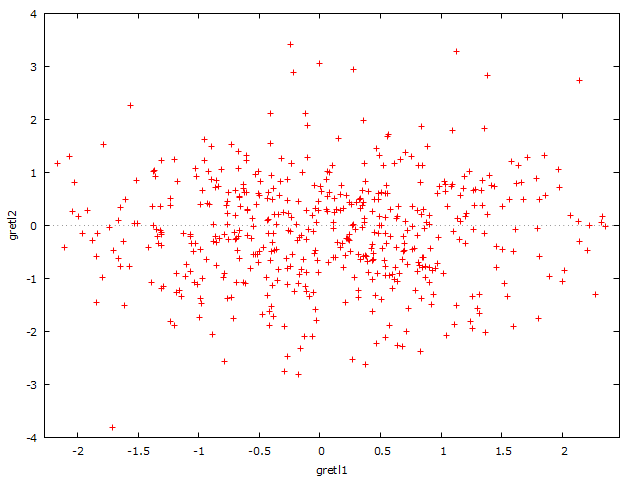
\includegraphics[width=0.9\textwidth,height=0.9\textheight]{gretlR/gretlR/scatter.png}

}

\caption{\label{fig-graph}Gretl graph}

\end{figure}

or the line graph:

\begin{Shaded}
\begin{Highlighting}[]
\InformationTok{\textasciigrave{}\textasciigrave{}\textasciigrave{}\{r,eval=TRUE\}}
\CommentTok{\#| label: fig{-}graph1}
\CommentTok{\#| fig{-}cap: Another Gretl graph}
\CommentTok{\#| out{-}width: 90\%}
\CommentTok{\#| out{-}height: 90\%}
\FunctionTok{include\_graph}\NormalTok{(}\AttributeTok{chunk =} \StringTok{"gretlR"}\NormalTok{,}\AttributeTok{graph =} \StringTok{"line.png"}\NormalTok{)}
\InformationTok{\textasciigrave{}\textasciigrave{}\textasciigrave{}}
\end{Highlighting}
\end{Shaded}

\begin{figure}[H]

{\centering 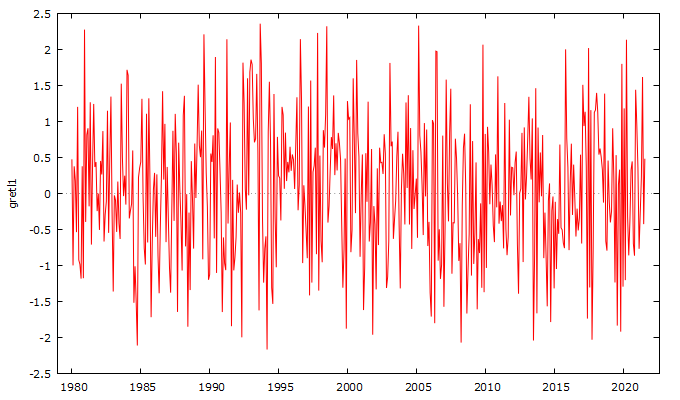
\includegraphics[width=0.9\textwidth,height=0.9\textheight]{gretlR/gretlR/line.png}

}

\caption{\label{fig-graph1}Another Gretl graph}

\end{figure}

\hypertarget{include_tex-function}{%
\section{include\_tex function}\label{include_tex-function}}

we can also include the equation of the OLS generated by the
\texttt{gretl} chunk and save as \texttt{olsEquation.tex}.

If the output is \texttt{pdf}, one can use the raw \texttt{LaTeX} codes
as follows:

\texttt{\textbackslash{}input\{gretlr/gretlR/olsEquation.tex\}}

Or use \texttt{include\_tex} function to include the equation as shown
below:

\begin{Shaded}
\begin{Highlighting}[]
\FunctionTok{include\_tex}\NormalTok{(}\AttributeTok{chunk =} \StringTok{"gretlR"}\NormalTok{,}\AttributeTok{tex =} \StringTok{"olsEquation"}\NormalTok{)}
\end{Highlighting}
\end{Shaded}

Or include lines 7 to 24 of \texttt{olsTable.tex} produced by the gretl
chunk:

\begin{Shaded}
\begin{Highlighting}[]
\InformationTok{\textasciigrave{}\textasciigrave{}\textasciigrave{}\{r,eval=TRUE\}}
\FunctionTok{include\_tex}\NormalTok{(}\AttributeTok{chunk =} \StringTok{"gretlR"}\NormalTok{,}\AttributeTok{tex =} \StringTok{"olsTAble"}\NormalTok{,}\AttributeTok{start =}\DecValTok{8}\NormalTok{,}\AttributeTok{end =} \DecValTok{24}\NormalTok{)}
\InformationTok{\textasciigrave{}\textasciigrave{}\textasciigrave{}}
\end{Highlighting}
\end{Shaded}

\begin{tabular}{lr@{.}lr@{.}lr@{.}lr@{.}l}
  &
 \multicolumn{2}{c}{Coefficient} &
  \multicolumn{2}{c}{Std.\ Error} &
   \multicolumn{2}{c}{$t$-ratio} &
    \multicolumn{2}{c}{p-value} \\[1ex]
const &
  0&0610266 &
    0&0431785 &
      1&413 &
        0&1582 \\
gretl2 &
  0&0239587 &
    0&0420559 &
      0&5697 &
        0&5691 \\
\end{tabular}


The OLS table output is saved by the \texttt{gretl} chunk as
\texttt{olsTable.Rmd}. The entire OLS table output can included as child
document as follows:

\begin{center}

Model 1: OLS, using observations 1980:01--2021:08 ($T$ = 500)\\
Dependent variable: gretl1\\

\vspace{1em}

\begin{tabular}{lr@{.}lr@{.}lr@{.}lr@{.}l}
  &
 \multicolumn{2}{c}{Coefficient} &
  \multicolumn{2}{c}{Std.\ Error} &
   \multicolumn{2}{c}{$t$-ratio} &
    \multicolumn{2}{c}{p-value} \\[1ex]
const &
  0&0610266 &
    0&0431785 &
      1&413 &
        0&1582 \\
gretl2 &
  0&0239587 &
    0&0420559 &
      0&5697 &
        0&5691 \\
\end{tabular}

\vspace{1ex}
\begin{tabular}{lrlr}
Mean dependent var &  0.058464 & S.D. dependent var &  0.959598 \\
Sum squared resid &  459.1937 & S.E. of regression &  0.960248 \\
$R^2$ &  0.000651 & Adjusted $R^2$ & -0.001355 \\
$F(1, 498)$ &  0.324542 & P-value($F$) &  0.569148 \\
Log-likelihood & $-$688.1853 & Akaike criterion &  1380.371 \\
Schwarz criterion &  1388.800 & Hannan--Quinn &  1383.678 \\
$\hat{\rho}$ & $-$0.046001 & Durbin--Watson &  2.091190 \\
\end{tabular}


\end{center}

\hypertarget{import_kable-function}{%
\section{import\_kable function}\label{import_kable-function}}

The \texttt{gretl} chunk also saves the OSL table as
\texttt{olsTable.csv}. The \texttt{import\_kable} function can be used
to import it as a table. further customisation can be done with
\texttt{kableExtra} package.

\begin{Shaded}
\begin{Highlighting}[]
\InformationTok{\textasciigrave{}\textasciigrave{}\textasciigrave{}\{r,eval=TRUE\}}
\FunctionTok{import\_kable}\NormalTok{(}\AttributeTok{chunk =} \StringTok{"gretlR"}\NormalTok{,}\AttributeTok{file =} \StringTok{"olsTAble.csv"}\NormalTok{,}
\AttributeTok{caption=}\StringTok{"Table generated from gretl chunk"}\NormalTok{, }
\AttributeTok{start=}\DecValTok{3}\NormalTok{,}\AttributeTok{end=}\DecValTok{7}\NormalTok{,}\AttributeTok{digits=}\DecValTok{2}\NormalTok{) }\SpecialCharTok{|\textgreater{}} 
\NormalTok{kableExtra}\SpecialCharTok{::}\FunctionTok{kable\_styling}\NormalTok{(}\AttributeTok{latex\_options =} \FunctionTok{c}\NormalTok{(}\StringTok{"basic"}\NormalTok{,}\StringTok{"hold\_position"}\NormalTok{,}\StringTok{"scale\_down"}\NormalTok{)) }\SpecialCharTok{|\textgreater{}}
\NormalTok{ kableExtra}\SpecialCharTok{::}\FunctionTok{row\_spec}\NormalTok{(}\DecValTok{0}\NormalTok{,}\AttributeTok{bold=}\NormalTok{T)}
\InformationTok{\textasciigrave{}\textasciigrave{}\textasciigrave{}}
\end{Highlighting}
\end{Shaded}

\begin{table}[!h]
\centering
\caption{Table generated from gretl chunk}
\centering
\resizebox{\ifdim\width>\linewidth\linewidth\else\width\fi}{!}{
\begin{tabular}[t]{l|r|r|r|r}
\hline
\textbf{} & \textbf{coefficient} & \textbf{std. error} & \textbf{t-ratio} & \textbf{p-value}\\
\hline
const & 0.06 & 0.04 & 1.41 & 0.16\\
\hline
gretl2 & 0.02 & 0.04 & 0.57 & 0.57\\
\hline
\end{tabular}}
\end{table}

\hypertarget{write_inp-function}{%
\section{write\_inp function}\label{write_inp-function}}

This function writes \texttt{gretl} file.

\begin{Shaded}
\begin{Highlighting}[]
\NormalTok{code}\OtherTok{=}\NormalTok{r}\StringTok{\textquotesingle{}(nulldata 500}
\StringTok{set seed 13}
\StringTok{gretl1 = normal()}
\StringTok{gretl2 = normal()}
\StringTok{setobs 12 1980:01 {-}{-}time{-}series}
\StringTok{gnuplot gretl1 {-}{-}time{-}series {-}{-}with{-}lines {-}{-}output="line.png"}
\StringTok{gnuplot gretl2 gretl1 {-}{-}output="scatter.png"}
\StringTok{)\textquotesingle{}}

\FunctionTok{write\_inp}\NormalTok{(code,}\AttributeTok{path=}\StringTok{"gretlCodes"}\NormalTok{)}
\end{Highlighting}
\end{Shaded}

\hypertarget{exec_inp-function}{%
\section{exec\_inp function}\label{exec_inp-function}}

This function executes existing \texttt{gretl} files.

\begin{Shaded}
\begin{Highlighting}[]
\NormalTok{code}\OtherTok{=}\NormalTok{r}\StringTok{\textquotesingle{}(nulldata 500}
\StringTok{set seed 13}
\StringTok{gretl1 = normal()}
\StringTok{gretl2 = normal()}
\StringTok{setobs 12 1980:01 {-}{-}time{-}series}
\StringTok{gnuplot gretl1 {-}{-}time{-}series {-}{-}with{-}lines {-}{-}output="line.png"}
\StringTok{gnuplot gretl2 gretl1 {-}{-}output="scatter.png"}
\StringTok{ )\textquotesingle{}}
\FunctionTok{write\_inp}\NormalTok{(code,}\AttributeTok{path=}\StringTok{"SomeFolder/gretlCodes"}\NormalTok{)}
\FunctionTok{exec\_inp}\NormalTok{(}\StringTok{"someFolder/gretlCodes"}\NormalTok{)}
\end{Highlighting}
\end{Shaded}

\hypertarget{exec_gretl-function}{%
\section{exec\_gretl function}\label{exec_gretl-function}}

This function creates \texttt{gretl}file from R object or a set of
character strings and executes it. It is a combination of
\texttt{write\_inp} and \texttt{exec\_inp} functions.

\begin{Shaded}
\begin{Highlighting}[]
\NormalTok{code}\OtherTok{=}\NormalTok{r}\StringTok{\textquotesingle{}(nulldata 500}
\StringTok{set seed 13}
\StringTok{gretl1 = normal()}
\StringTok{gretl2 = normal()}
\StringTok{setobs 12 1980:01 {-}{-}time{-}series}
\StringTok{gnuplot gretl1 {-}{-}time{-}series {-}{-}with{-}lines {-}{-}output="line.png"}
\StringTok{gnuplot gretl2 gretl1 {-}{-}output="scatter.png"}
\StringTok{ )\textquotesingle{}}
\FunctionTok{exec\_gretl}\NormalTok{(code)}
\end{Highlighting}
\end{Shaded}

\hypertarget{demo}{%
\section{Demo}\label{demo}}

Demo can be accessed via \texttt{demo(package="gretlR")}.

\begin{Shaded}
\begin{Highlighting}[]
\FunctionTok{demo}\NormalTok{(exec\_inp) }
\FunctionTok{demo}\NormalTok{(write\_inp)}
\FunctionTok{demo}\NormalTok{(exec\_gretl)}
\end{Highlighting}
\end{Shaded}

\hypertarget{r-markdown-template}{%
\section{R Markdown template}\label{r-markdown-template}}

The R Markdown template for the \texttt{gretlR} can be accessed via
\texttt{file\ -\textgreater{}\ New\ File\ -\textgreater{}\ R\ Markdown\ -\textgreater{}\ From\ Template\ -\textgreater{}\ gretlR}

\hypertarget{similar-packages}{%
\section{Similar Packages}\label{similar-packages}}

Similar packages include
\href{https://github.com/sagirumati/DynareR}{DynareR} (Mati, 2020a,
2022a), \href{https://github.com/sagirumati/gretlR}{EviewsR} (Mati,
2020b, 2022b; Mati et al., 2023), and
\href{https://github.com/sagirumati/URooTab}{URooTab} (Mati, 2023b,
2023a)

For further details, consult Mati (2020c) and Mati (2022c).

Please download a set of example files from
\href{https://github.com/sagirumati/gretlR/tree/master/inst/examples/}{Github}.

\hypertarget{references}{%
\section*{References}\label{references}}
\addcontentsline{toc}{section}{References}

\hypertarget{refs}{}
\begin{CSLReferences}{1}{0}
\leavevmode\vadjust pre{\hypertarget{ref-Mati2020}{}}%
Mati, S. (2020a). DynareR: Bringing the power of dynare to {R, R
Markdown, and Quarto}. \emph{CRAN}.
\url{https://CRAN.R-project.org/package=DynareR}

\leavevmode\vadjust pre{\hypertarget{ref-Mati2020a}{}}%
Mati, S. (2020b). \emph{EviewsR: A seamless integration of {EViews} and
{R}}. \url{https://CRAN.R-project.org/package=EviewsR}

\leavevmode\vadjust pre{\hypertarget{ref-Mati2020b}{}}%
Mati, S. (2020c). \emph{gretlR: A seamless integration of {Gretl} and
{R}}. \url{https://CRAN.R-project.org/package=gretlR}

\leavevmode\vadjust pre{\hypertarget{ref-mati2022dynarer}{}}%
Mati, S. (2022a). \emph{Package {``DynareR''}}.
\url{https://cran.r-project.org/web/packages/DynareR/DynareR.pdf}

\leavevmode\vadjust pre{\hypertarget{ref-mati2022eviewsr}{}}%
Mati, S. (2022b). \emph{Package {``EviewsR''}}.
\url{https://cran.r-project.org/web/packages/EviewsR/EviewsR.pdf}

\leavevmode\vadjust pre{\hypertarget{ref-mati2022gretlr}{}}%
Mati, S. (2022c). \emph{Package {``gretlR''}}.
\url{https://cran.r-project.org/web/packages/gretlR/gretlR.pdf}

\leavevmode\vadjust pre{\hypertarget{ref-mati2023urootab}{}}%
Mati, S. (2023a). \emph{Package {``URooTab''}}.
\url{https://cran.r-project.org/web/packages/URooTab/URooTab.pdf}

\leavevmode\vadjust pre{\hypertarget{ref-Mati2023a}{}}%
Mati, S. (2023b). \emph{{URooTab}: Tabular reporting of {EViews} unit
root tests}. \url{https://github.com/sagirumati/URooTab}

\leavevmode\vadjust pre{\hypertarget{ref-Mati2023}{}}%
Mati, S., Civcir, I., \& Abba, S. I. (2023). {EviewsR}: An r package for
dynamic and reproducible research using {EViews}, r, r markdown and
quarto. \emph{The R Journal}, \emph{15}(2), 169--205.
\url{https://doi.org/10.32614/rj-2023-045}

\end{CSLReferences}



\end{document}
